
\section{Discussion}

\subsection{Sources of computational efficiency}

The numerical results indicate that the computational advantage of the proposed framework arises from exploiting the structure of lower-bound FELA at several computational levels.

At the linear-algebra level, the repeated linear systems arising in ADMM permit expensive sparse factorizations to be reused across iterations, resulting in a substantially lower cost per iteration than that of the IPM solvers. At the conic-constraint level, active-cone identification exploits the fact that only a subset of the local yield constraints governs the solution near collapse, allowing the penalty weights to be adapted selectively. At the mesh-sequence level, coarse-to-fine warm-starting transfers information between closely related FELA problems and reduces the transient phase of convergence. Finally, the dominant linear algebra, projection, and vector operations are mapped onto the GPU, further reducing the cost of each ADMM iteration.

These mechanisms are complementary. Warm-starting primarily improves the initial iterate, active-cone identification improves convergence during the later stages of the solve, and GPU acceleration reduces the computational cost of carrying out each iteration. The combined effect is therefore a large reduction in overall time-to-solution especially as the problem size increases.

\subsection{Scalability bottleneck of direct factorization in 3D}
\label{sec:3D_scalability}

The principal scalability limitation of the current 3D implementation arises from fill-in during sparse direct factorization. Although the ADMM iterations remain relatively inexpensive in terms of iteration count, the linear systems generated by three-dimensional FELA become substantially more demanding as the mesh is refined. This behaviour is primarily associated with the different sparsity structure of the 3D formulation.

In lower-bound FELA, the 3D discretization introduces stronger and more spatially extensive coupling than its 2D counterpart. Each stress point contains more stress components, the intra-element equilibrium conditions increase from two equations per stress point in 2D to three in 3D, and the dimension of the SOC blocks increases from three to six for the Drucker--Prager or von Mises formulations considered here. Together with the increased connectivity of three-dimensional finite-element meshes, these larger local blocks lead to a more strongly coupled constraint matrix, as illustrated by the sparsity patterns in Figure~\ref{fig:A_sparsity}.

\begin{figure}
    \centering
    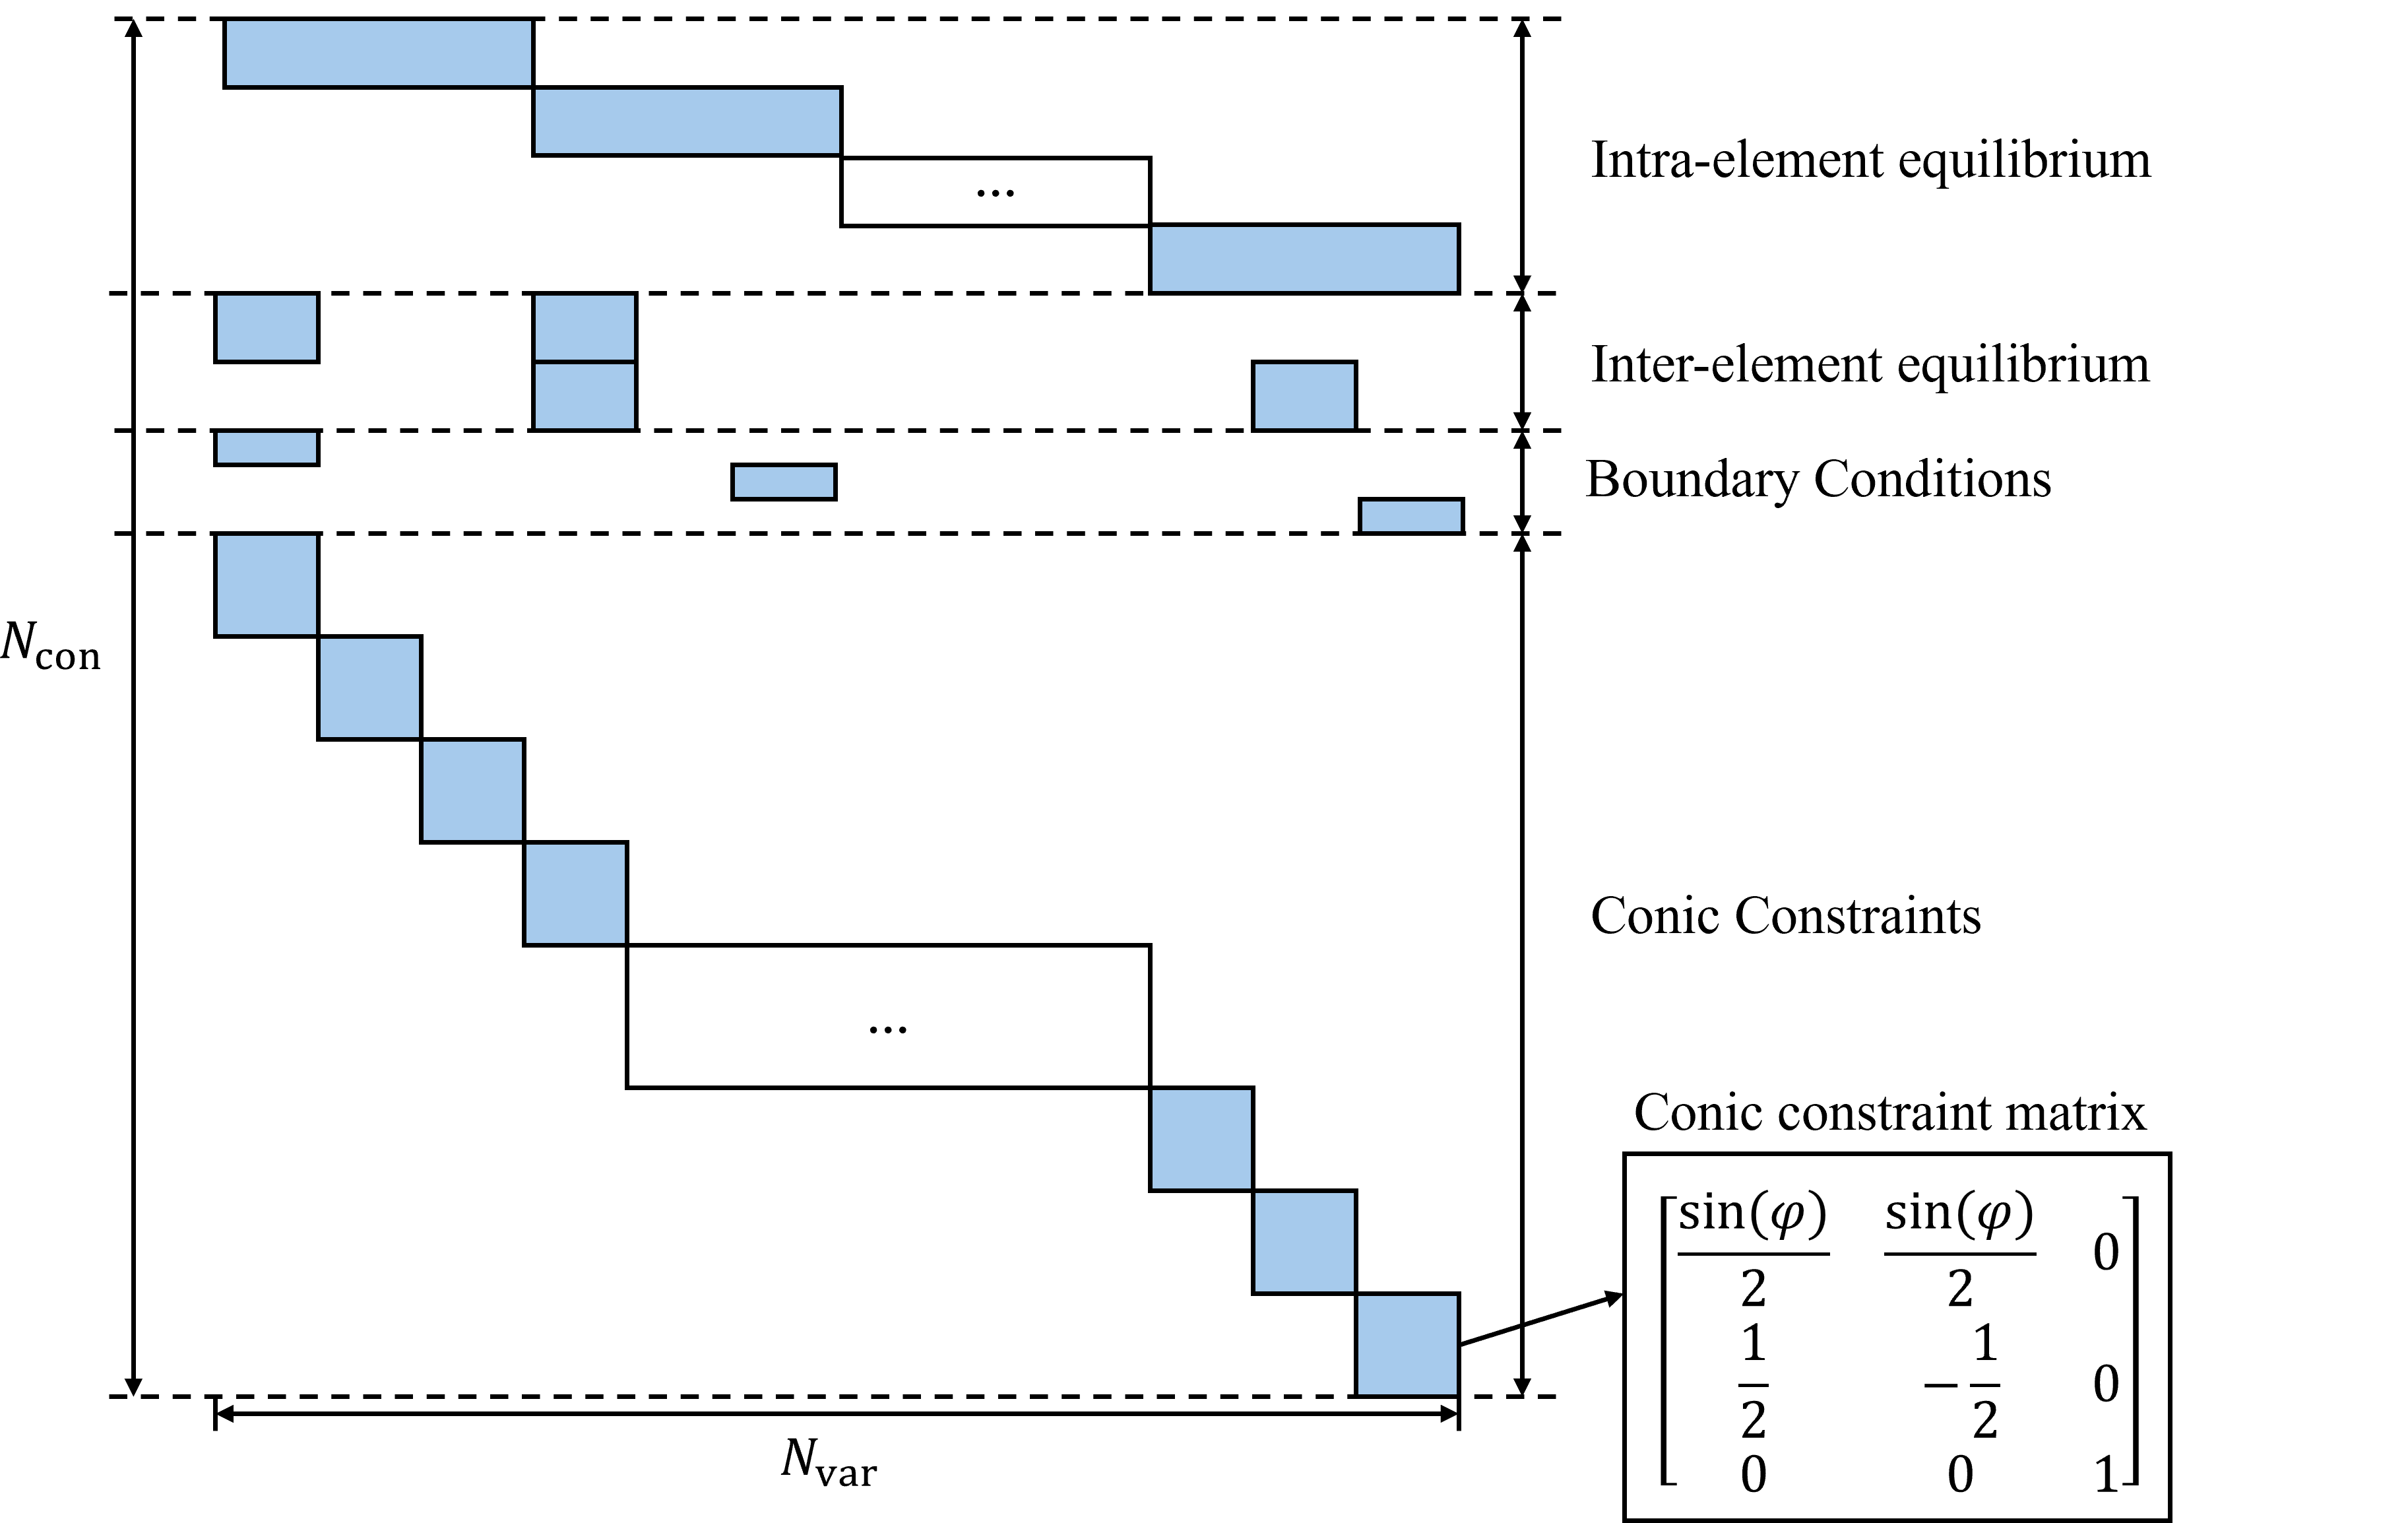
\includegraphics[width=0.8\textwidth]{figures/Res_To_Date/A_sparsity.png}
    \caption{Sparsity patterns of the constraint matrix $A$ in the 2D and 3D FELA formulations.}
    \label{fig:A_sparsity}
\end{figure}

The stronger coupling in the 3D system leads to substantially more fill-in during reordering and factorization. As a result, the numerical factors become significantly larger, increasing both the memory required to store them and the computational cost of the associated sparse linear algebra. In particular, the numerical factorization required whenever the system matrix is updated becomes more expensive, while the repeated triangular solves performed at each ADMM iteration also incur a higher cost.

Consequently, the computational expense of large 3D problems is not determined solely by the number of ADMM iterations. As the factors grow and approach the available GPU memory capacity, memory traffic, data movement, and the cost of operating on the enlarged sparse factors increasingly dominate the overall solution time. This effect can be substantial even when the 2D and 3D problems contain a comparable number of optimization variables, since sparse-factorization cost depends strongly on the sparsity pattern and the resulting fill-in rather than on the system dimension alone.

This explains why the direct GPU-based approach remains highly efficient for the 2D plane-strain benchmarks considered here, while its scalability becomes increasingly constrained by sparse direct factorization in large-scale 3D discretizations. The observed bottleneck therefore motivates the consideration of indirect or matrix-free linear-solver strategies, as discussed in the following section.

\subsection{Potential of indirect and matrix-free ADMM solvers}


Nevertheless, a more scalable direction may be to avoid explicitly computing and storing the sparse factorization altogether, and instead adopt an indirect linear solution strategy within ADMM. This is especially relevant for three-dimensional FELA, where direct factorization of sparse matrices can quickly become unfavourable due to excessive fill-in~\cite{Shewchuk_CG}. As noted in the broader numerical linear algebra literature, iterative solvers are often preferable, and in many large-scale three-dimensional applications practically necessary, due to the memory and computational costs associated with sparse direct methods~\cite{Saad_book}. Several ADMM-based solvers already provide indirect linear-system solvers~\cite{SCS, OSQP, COSMO, GeNIOS}. Notably, SCS has reported speedups from its GPU-based indirect implementation on large-scale problems~\cite{SCS}, suggesting that the combination of ADMM and indirect solves can be practical and scalable for sufficiently large instances.


\subsection{Generality, limitations, and future extensions}

The proposed method achieves a speedup over the IPM on many large-scale problems arising in FELA, while maintaining accuracy comparable to MOSEK under a similar accuracy target. We note, however, that part of this speedup is achieved using a GPU-based implementation, whereas MOSEK is run on a multi-threaded CPU. 

While the proposed acceleration techniques are developed in the context of LB-FELA, they target generic bottlenecks of first-order methods for SOCPs. Therefore, they may also benefit other sparse SOCPs with PDE-like structures. A systematic evaluation on broader classes of problems is left for future work.


Apart from the GPU-accelerated ADMM solver itself, the integration with adaptive mesh refinement enables the computational effort to be concentrated in the regions most relevant to the collapse mechanism, leading to tighter lower-bound solutions without uniformly refining the entire domain.

Future work will also consider more advanced yield criteria, such as Mohr-Coulomb and Lade-Duncan. Incorporating these criteria would increase the practical value of the proposed methodology, as they are widely used in geotechnical and engineering applications. Within the ADMM framework, such criteria can be incorporated provided that the projection of a general stress state onto the admissible yield surface can be computed efficiently~\cite{daSilva_2020, 3DLD}. For example, although not necessarily in the context of FELA, Clausen and co-workers implemented the three-dimensional Mohr-Coulomb criterion using a return-mapping strategy, in which the stress state is transformed into principal stress space, projected onto the yield surface, and then transformed back to the original stress space~\cite{Clausen_2007}. Extending this type of projection strategy to the present FELA-ADMM framework is a promising direction for future research.




